\documentclass[12pt, a4paper]{article}
\title{Резонанс напряжений (3.2.2)}
\author{Стеценко Георгий, Б02-312}
\date{}
% !TeX encoding = UTF-8

\usepackage{geometry}
\usepackage{amsmath, amsfonts, amssymb, amsthm} % стандартный набор AMS-пакетов для математ. текстов
\usepackage{mathtext}
\usepackage[utf8]{inputenc} % кодировка utf8
\usepackage[russian]{babel} % русский язык
\usepackage[pdftex,dvipsnames]{xcolor} % работа с цветами
\usepackage[pdftex]{graphicx} % графика (картинки)
\usepackage{tikz,pgfplots} % рисунки
\usepackage{indentfirst}
%\usepackage[labelfont=bf,labelsep=endash,skip=3pt]{caption} % подпись картинок
% \usepackage{fancyhdr,pageslts} % настройка колонтитулов
\usepackage{enumitem} % работа со списками
\usepackage{floatrow,multicol,multirow,longtable,hhline} % работа с таблицами
\usepackage{float,wrapfig} % плавающие объекты
\usepackage{tcolorbox} % рамка вокруг текста
%\usepackage[calc]{datetime2} % дата
\usepackage{bm} % жирное начертание в формулах
\usepackage{physics} % физический пакет
\DeclareMathAlphabet\mathbfcal{OMS}{cmsy}{b}{n}
\usepackage{pgfornament} % красивые рюшечки и вензеля
\usepackage{mdframed}
\usepackage{derivative}
\usepackage{mathrsfs} %EDS
\usepackage{soul} % strikethorugh
%\usepackage{boondox-cal}

% ----------------------------------------
% Настройка шрифта

% Просто закооментируйте следующую строчку, если не работает. Будет другой шрифт, правда :(
% \usepackage{pscyr}

% ----------------------------------------
% Стилевые настройки

\usepackage{boldline} % жирная линия после таблиц (чтобы не было ошибок, этот пакет должен подключаться именно тут!)
\floatsetup[table]{style=Plaintop,floatrowsep=qquad} % настройка оформления таблиц
\setlist[enumerate,itemize]{leftmargin=5mm,itemindent=10mm,itemsep=0mm,
listparindent=0em,labelsep=2mm,topsep=2mm,labelwidth=4mm} % настройки списков

\setlength{\columnsep}{0.5cm} % расстояние между колонками
\setlength{\parskip}{1pt} % расстояние до текста от колонтитула

%\usepackage{titlesec} % управление оформлением section
%\renewcommand{\thesection}{\Roman{section}}
%\titleformat{\section}[block]{\bfseries\large}{\thesection.}{5pt}{}

% ----------------------------------------
% Настройки полей
\geometry{
  left=10mm,
  top=10mm,
  right=10mm,
  bottom=15mm,
  marginparsep=0mm,
  marginparwidth=0mm,
  headheight=0pt,
  headsep=0pt,
footskip=20pt}

% ----------------------------------------
% Настройки колонтитулов и нумерации страниц
\pagenumbering{arabic}



\newcounter{ntask}
\setcounter{ntask}{0}


\newcommand{\arsh}{\mathrm{arsh} \,\,}
\newcommand{\arch}{\mathrm{arch} \,\,}
\newcommand{\arth}{\mathrm{arth} \,\,}
\newcommand{\arcth}{\mathrm{arcth} \,\,}
\renewcommand{\Re}{\operatorname{Re} \,}
\newcommand{\EDS}{\mathscr{E}}
\newcommand{\diffract}[1]{\frac{\mathrm{d}#1}{\mathrm{d}t}}

\begin{document}
\maketitle

\section{Цель работы}
Исследование резонанса напряжений в~последовательном
колебательном контуре с~изменяемой ёмкостью, получение амплитудно­
частотных и~фазово-частотных характеристик, определение основных па­
раметров контура.

\section{Теоретические сведения}
При анализе цепей переменного тока вводится понятие комплексной амплитуды, которая позволяет связать напряжение и~ток при~установившихся гармонических колебаниях в~цепи. Пусть мгновенные значения тока и~напряжения на~некотором элементе равны:

$$ i = I_A \cos(\omega t),~u = U_A \cos (\omega t + \varphi)$$
Тогда можно ввести комплексные ток и~напряжение, равные соответственно:
$$\hat{I} = I_A e^{j\omega t}, \hat{U} = U_A e^{j(\omega t + \varphi)}$$
Тогда $i=\Re \hat{I}$, $u = \Re \hat{U}$, и~элемент описывается своим импедансом, равным соответственно:
$$\hat{Z} := \frac{\hat{U}}{\hat{I}}$$
Для~идеальных сопротивления R, индуктивности L и~ёмкости C известны стандартные формулы импеданса, которые получаются из уравнений $u_R = i_R \cdot R$, $u_L = L\diffract{i_L}$, $i_C = C\diffract{u_C}$:
$$ \hat{Z_R} = R$$
$$\hat{Z_C} = \frac{1}{j\omega C} = -j \frac{1}{\omega C}$$
$$\hat{Z_L} = j\omega L$$

\begin{wrapfigure}[13]{r}{3.5cm}\vspace{-15mm}
  \centering
  \begin{tikzpicture}
    \draw [step=1, dashed, very thin] (-0.5, -1.5) grid (2.5, 3.5);
    \draw [->, thick] (0,0) -- (2,0) node [anchor=south west] {$\hat{I}$};
    \draw [->, very thick] (0,0) -- (1,0) node [anchor=south west] {$\hat{U_R}$};
    \draw [->, very thick] (0,0) -- (0,3) node [anchor=south west] {$\hat{U_L}$};
    \draw [->, very thick] (0,0) -- (0,-1) node [anchor=south west] {$\hat{U_C}$};
    \draw [->, very thick] (0,0) -- (1, 2) node [anchor=south west] {$\hat{U}$};
    \draw (0.5, 0) arc (0:63.4:0.5);
    \draw (35:0.75) node {$\delta$};
  \end{tikzpicture}
  \caption{Векторная диаграмма напряжений}
  \label{udiag}
\end{wrapfigure}
В любой момент времени выполнены законы Кирхгофа для~мгновенных значений тока и~напряжения, а~значит, они выполнены и~в~комплексном смысле. Поэтому при~расчётах RLC-цепей можно использовать комплексные аналоги вещественных формул для~расчёта цепей из~сопротивлений. К~примеру, при~последовательном соединении трёх элементов с импедансами $\hat{Z_1}$, $\hat{Z_2}$, $\hat{Z_3}$ эквивалентный импеданс участка будет равен $\widehat{Z_{123}} = \hat{Z_1} + \hat{Z_2} + \hat{Z_3}$.

Изобразим векторную диаграмму напряжений в~последовательном RLC-участке (\textit{Рис. \ref{udiag}}).
Поймём, что $\hat{Z_R} (\omega)  = \text{const}$, $\hat{Z_L} (\omega) >0$~и~возрастает, $\hat{Z_С} (\omega)<0$~и~возрастает, то есть существует такое $\omega_0$, что $\widehat{Z_{RLC}} = R + 0j$. Так как $\Re(\hat U) \equiv |\hat I| R$, $|\hat U| \geq |\hat I|R$, и минимум достигается при $\omega = \omega_0$. Он и называется \textbf{резонансом напряжений}.

Резонанс напряжений определяется из условия $\hat{Z_C} = -\hat{Z_L}$, то~есть:

\begin{equation}
  \omega_0 = \sqrt{\frac{1}{LC}}
  \label{omega0}
\end{equation}

\newpage
\renewcommand{\labelenumi}{(\alph{enumi})}
Цепь содержит в~себе неидеальные элементы~--- резисторы, катушки индуктивности, и~конденсаторы. Обсудим, какие особенности это вносит в~наш эксперимент.
\begin{enumerate}
  \item \textbf{Катушка индуктивности}

    Катушка индуктивности имеет некоторую межвитковую ёмкость $C_L$, а~так~же сопротивление обмотки $R_L$. Для нашей катушки известно, что собственная частота резонанса $\nu_L \sim 1\text{MHz}$, то есть реактивная составляющая импеданса может быть выражена через эффективную индуктивность $L(\omega) = L_{stat} (1-(\nu/\nu_0)^2)$. Мы же будем работать в диапазоне $\nu \leq 50 \text{kHz} \ll \nu_L$, и~посему будем пренебрегать межвитковой ёмкостью, и, соответственно, изменением эффективной индуктивности. Тем~не~менее, мы будем учитывать активную составляющую импеданса катушки.

  \item \textbf{Конденсатор}

    Полипропиленовые конденсаторы в данной работе в рабочем диапазоне частот имеют пренебрежимо малые индуктивности. Однако, необходимо учесть так назвыаемое эквивалентное последовательное сопротивление $R_S$, обусловленное, в основном, сопротивлением материала обкладок.
\end{enumerate}

Таким образом, эквивалентные параметры цепи $R_\Sigma = R + R_L + R_S$, $L_\Sigma = L$, $C_\Sigma = C$.

Нам так же понадобится понятие добротности колебательного контура, определяемое как ${Q := \omega_0 \frac{W}{P_d}}$, где $\omega_0$ --- собственная (резонансная) частота, $W$ --- энергия, запасённая в системе, $P_d$ --- рассеиваемая мощность. Знаем, что при слабом затухании $W = \frac 1 2 LI_A^2$, $P_d = \frac 1 2 I_A^2 R$, $\omega_0 = \frac{1}{\sqrt{LC}}$, тогда по определению:
\begin{equation}
  Q = \frac{1}{R} \sqrt{\frac L C} \quad \left(Q \gg 1\right)
  \label{Q}
\end{equation}
Несложно далее получить, что при $Q \gg 1$, если ширина пика на уровне $1/\sqrt 2$ от максимума равна $\Delta \omega$, то $Q \approx \frac{\omega_0}{\Delta\omega}$.

\section{Методика измерений}
\begin{wrapfigure}[12]{r}{8.4cm} \centering \vspace{-8mm}
  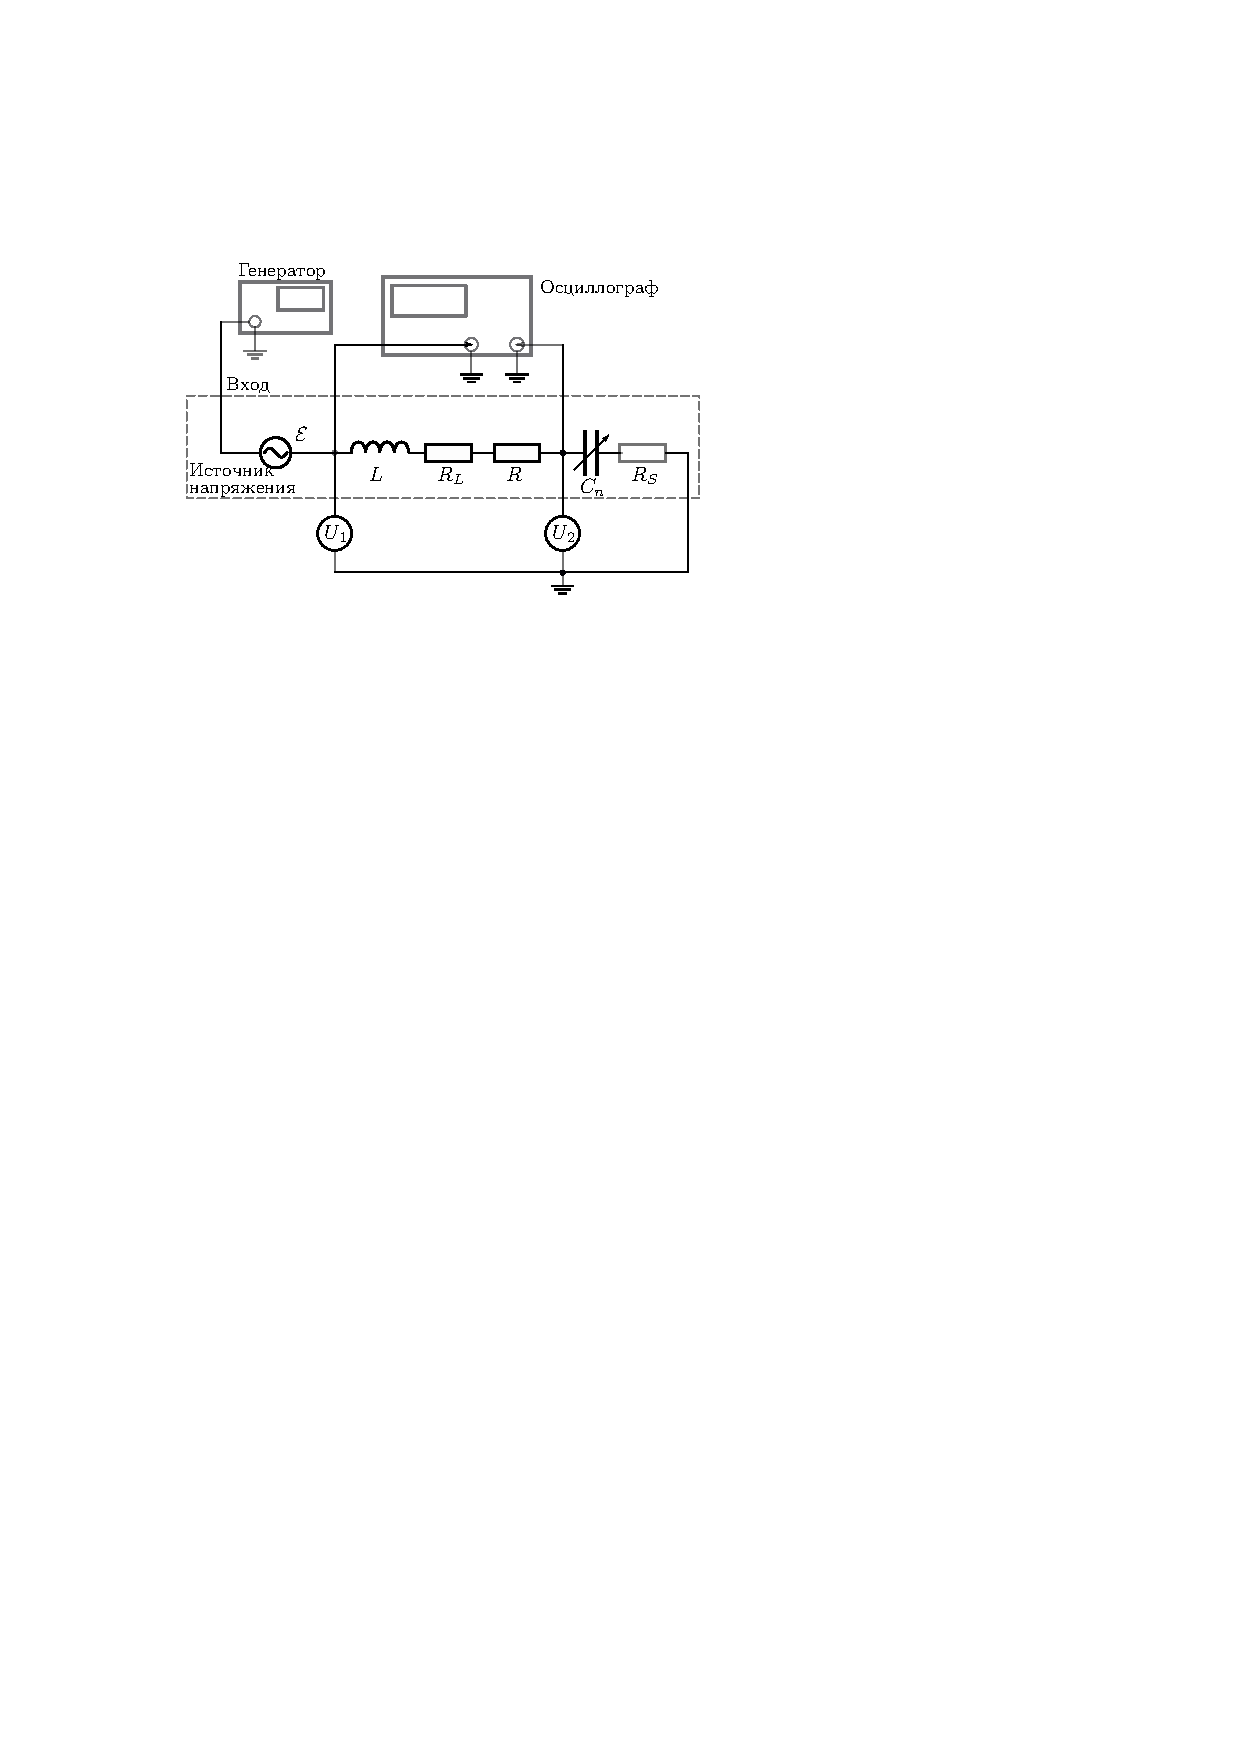
\includegraphics[width=8cm]{setup.pdf}
  \caption{Схема установки}
  \label{setup}
\end{wrapfigure}


\textbf{В работе используются:} осциллограф, 2 вольтметра, генератор, RLC-контур с источником питания.

Последовательный контур подключен к источнику напряжения, на который подается сигнал с генератора. На \textit{рис. \ref{setup}} изображена эквивалентная схема установки. Напряжения снимаются вольтметрами 1 и 2 со всей цепи и с конденсатора соответственно. Напряжение резистора R в цепи $R = 3.50~\mathrm{\Omega}$.

В начале были промерены все режимы RLC-черного ящика, и найдены резонансные частоты. Изменения напряжения менее чем на 1\% проигнорированы, из данных получены соответствующие параметры контура. Далее сняты АЧХ и ФЧХ колебательного контура, и проведены дальнейшие сравнения полученных зависимостей.

Как известно, при вынужденных колебаниях в колебательном контуре устанавливается вынуждающая частота. Источник питания работает на OpAmp, поэтому его рабочая частота в точности совпадает с частотой генератора. Таким образом, погрешностью определения частоты можно пренебречь.

\newpage
\section{Результаты измерений и~обработка данных}

\begin{table}[H]
  \begin{tabular}{|rrrr|r|rrrr|r|r|}
    \hline
    \multicolumn{1}{|c|}{$C_n, \text{nF}$} & \multicolumn{1}{c|}{$f_{0n}, \text{kHz}$} & \multicolumn{1}{c|}{$U_C, \text{V}$} & \multicolumn{1}{c|}{$\EDS, \text{V}$} & \multicolumn{1}{c|}{$L, \mathrm{\mu H}$} & \multicolumn{1}{c|}{Q}    & \multicolumn{1}{c|}{$\rho, \mathrm{\Omega}$} & \multicolumn{1}{c|}{$R_\Sigma, \mathrm{\Omega}$} & \multicolumn{1}{c|}{$R_{S_{max}}, \mathrm{\Omega}$} & \multicolumn{1}{c|}{$R_L, \mathrm{\Omega}$} & \multicolumn{1}{c|}{$I,.\text{mA}$} \\ \hline
    \multicolumn{1}{|r|}{24.8}             & \multicolumn{1}{r|}{32.43}                & \multicolumn{1}{r|}{1.39}            & 0.05                                  & 971.17                                   & \multicolumn{1}{r|}{27.8} & \multicolumn{1}{r|}{197.88}                  & \multicolumn{1}{r|}{7.12}                        & 0.198                                               & 3.62                                        & 7.02                                    \\ \hline
    \multicolumn{1}{|r|}{33.2}             & \multicolumn{1}{r|}{28.00}                & \multicolumn{1}{r|}{1.23}            & 0.05                                  & 973.16                                   & \multicolumn{1}{r|}{24.6} & \multicolumn{1}{r|}{171.21}                  & \multicolumn{1}{r|}{6.96}                        & 0.171                                               & 3.46                                        & 7.18                                    \\ \hline
    \multicolumn{1}{|r|}{47.6}             & \multicolumn{1}{r|}{23.41}                & \multicolumn{1}{r|}{1.06}            & 0.05                                  & 971.03                                   & \multicolumn{1}{r|}{21.2} & \multicolumn{1}{r|}{142.83}                  & \multicolumn{1}{r|}{6.74}                        & 0.142                                               & 3.24                                        & 7.42                                    \\ \hline
    \multicolumn{1}{|r|}{57.5}             & \multicolumn{1}{r|}{21.29}                & \multicolumn{1}{r|}{0.97}            & 0.05                                  & 971.90                                   & \multicolumn{1}{r|}{19.4} & \multicolumn{1}{r|}{130.01}                  & \multicolumn{1}{r|}{6.70}                        & 0.130                                               & 3.20                                        & 7.46                                    \\ \hline
    \multicolumn{1}{|r|}{68.0}             & \multicolumn{1}{r|}{19.58}                & \multicolumn{1}{r|}{0.90}            & 0.05                                  & 971.64                                   & \multicolumn{1}{r|}{18.0} & \multicolumn{1}{r|}{119.54}                  & \multicolumn{1}{r|}{6.64}                        & 0.120                                               & 3.14                                        & 7.53                                    \\ \hline
    \multicolumn{1}{|r|}{81.6}             & \multicolumn{1}{r|}{19.78}                & \multicolumn{1}{r|}{0.91}            & 0.05                                  & \st{793.41}                                   & \multicolumn{1}{r|}{18.2} & \multicolumn{1}{r|}{98.61}                   & \multicolumn{1}{r|}{5.42}                        & 0.099                                                & \st{1.92}                                        & 9.23                                    \\ \hline
    \multicolumn{1}{|r|}{102.8}            & \multicolumn{1}{r|}{15.92}                & \multicolumn{1}{r|}{0.76}            & 0.05                                  & 972.21                                   & \multicolumn{1}{r|}{15.2} & \multicolumn{1}{r|}{97.25}                   & \multicolumn{1}{r|}{6.40}                        & 0.097                                                & 2.90                                        & 7.82                                    \\ \hline
    \multicolumn{4}{|c|}{Среднее значение}                                                                                                                            & 971.85                                   & \multicolumn{4}{r|}{}                                                                                                                                                             & 3.26                                        &                                     \\ \hline
    \multicolumn{4}{|c|}{Случайная погрешность}                                                                                                                       & 0.71                                     & \multicolumn{4}{r|}{}                                                                                                                                                             & 0.23                                        &                                     \\ \hline
  \end{tabular}
  \caption{Результаты измерения резонансных частот}
  \label{dataall}
\end{table}

Отметим, что измерения 6-го контура, очевидно, являются выбросом (см. столбец $\textit{L}$ в табл. \ref{dataall}), соответственно надписи на рабочем блоке, и они проигнорированы при дальнейшей обработке.

Так как значения $L$ получаются из ур. (\ref{omega0}), $\varepsilon(L) = \sqrt{\varepsilon(C)^2 + 2 \varepsilon(f_0)^2}$. Так как $\varepsilon(f_0)$ мало,\newline ${\varepsilon(L) \approx \varepsilon(C) \lesssim \frac{0.1}{24.8} \approx 0.2 \%}$. Тогда $\sigma(L) = \sqrt{\sigma(L)_{сл}^2 + \sigma(L)_{ст}^2} \approx 2.1~\mathrm{\mu H}$. Тогда $L = (972 \pm 3)~\mathrm{\mu H}$.

\vspace{1.5em}

Теперь перейдём к измерениям на контурах с 1-м и 5-м конденсаторами при постоянном $\EDS$. Сырые данные к АЧХ и ФЧХ можно найти в \textbf{Приложении 1}. Здесь они приведены не будут для улучшения читаемости. Кроме того, на графиках АЧХ не будут отображены кресты погрешностей, так как они слишком малы, чтобы занимать значимое пространство на графике.

\begin{figure}[H]
  \centering
  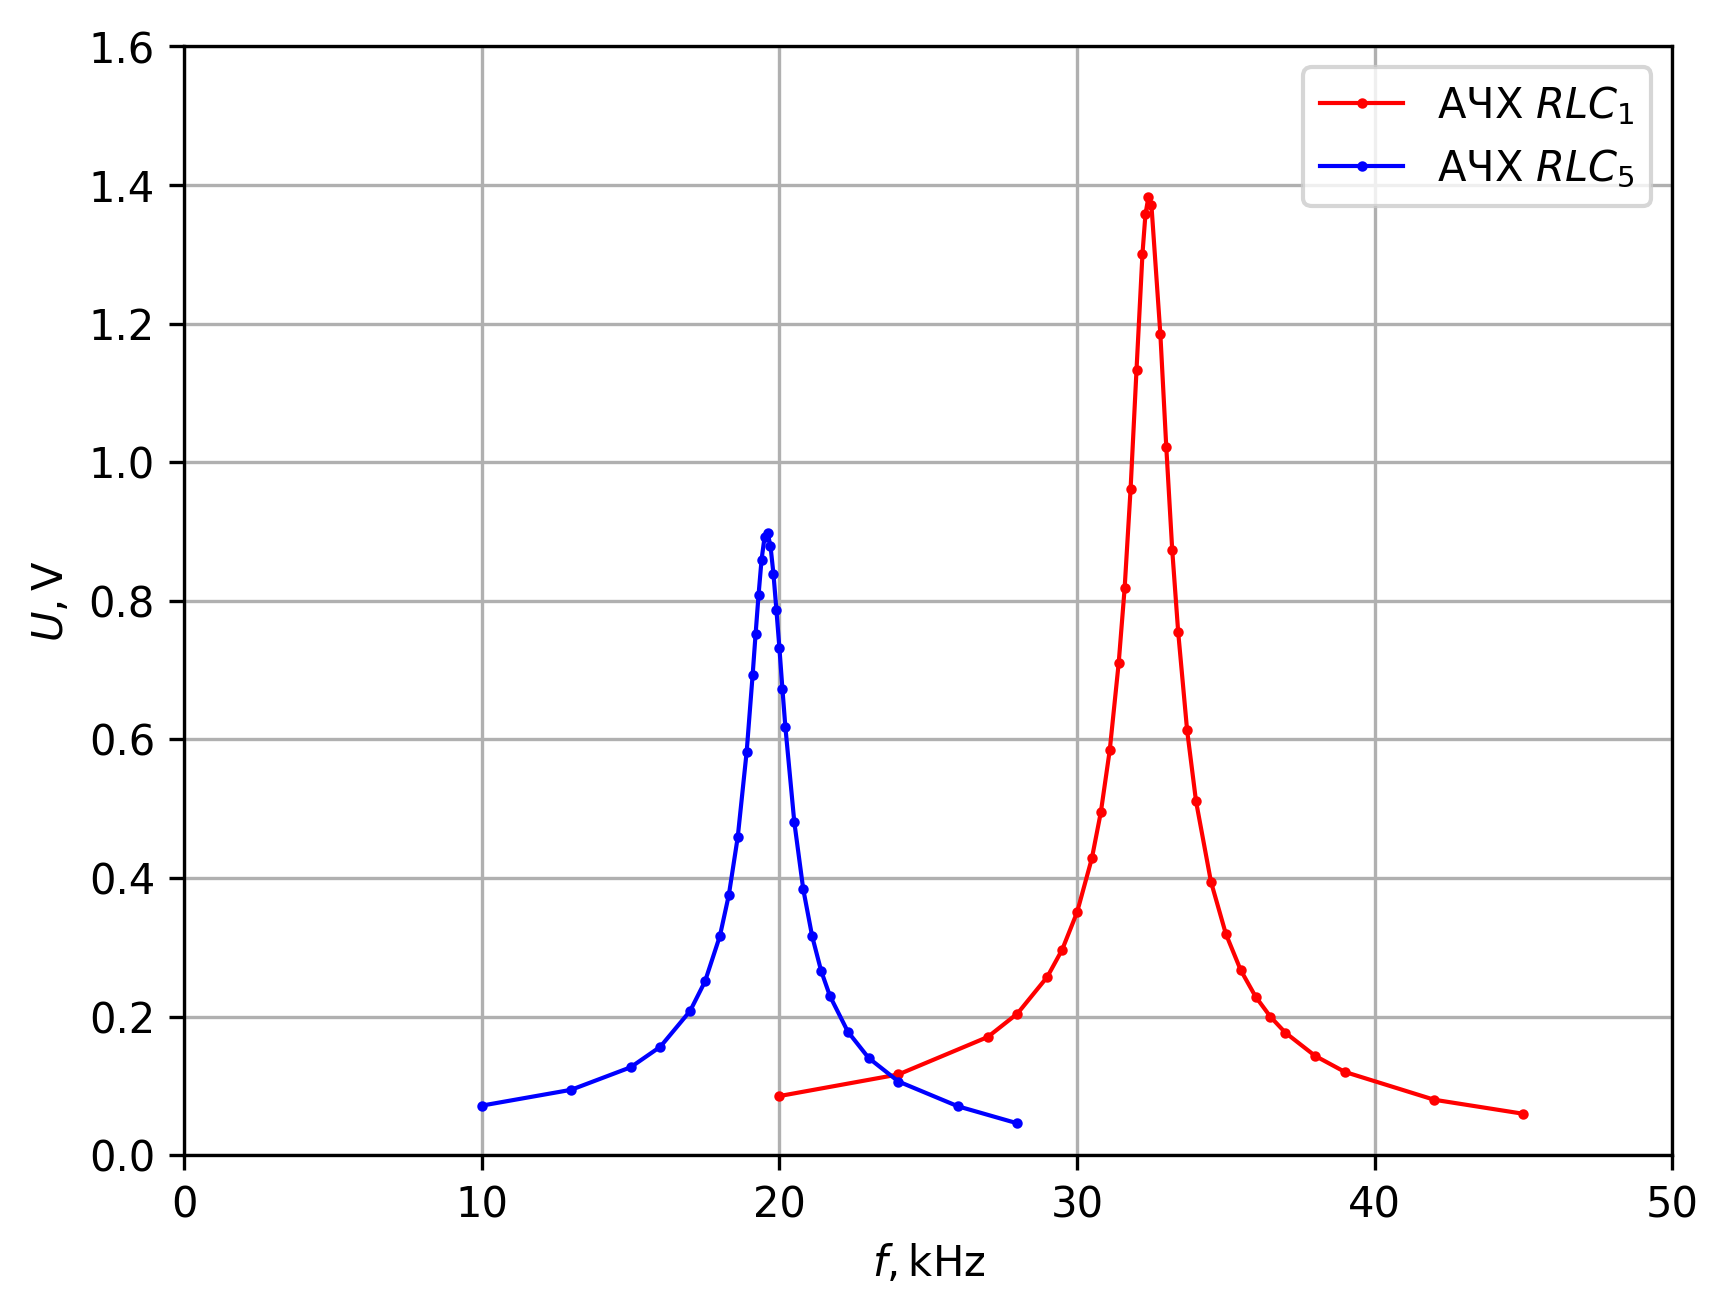
\includegraphics[width = 0.8\linewidth]{afc15.png}
  \caption{Сводный график АЧХ для контуров с 1-м и 5-м конденсаторами}
\end{figure}

По графику видно, что при прочих равных большая ёмкость конденсатора увеличивает период колебаний в контуре, но при этом уменьшает его добротность (меньшее напряжение при резонансе), что соответствует уравнениям (\ref{omega0}) и (\ref{Q}).

\newpage
Перёдем к детальному анализу АЧХ по отдельности.

\begin{figure}[H]
  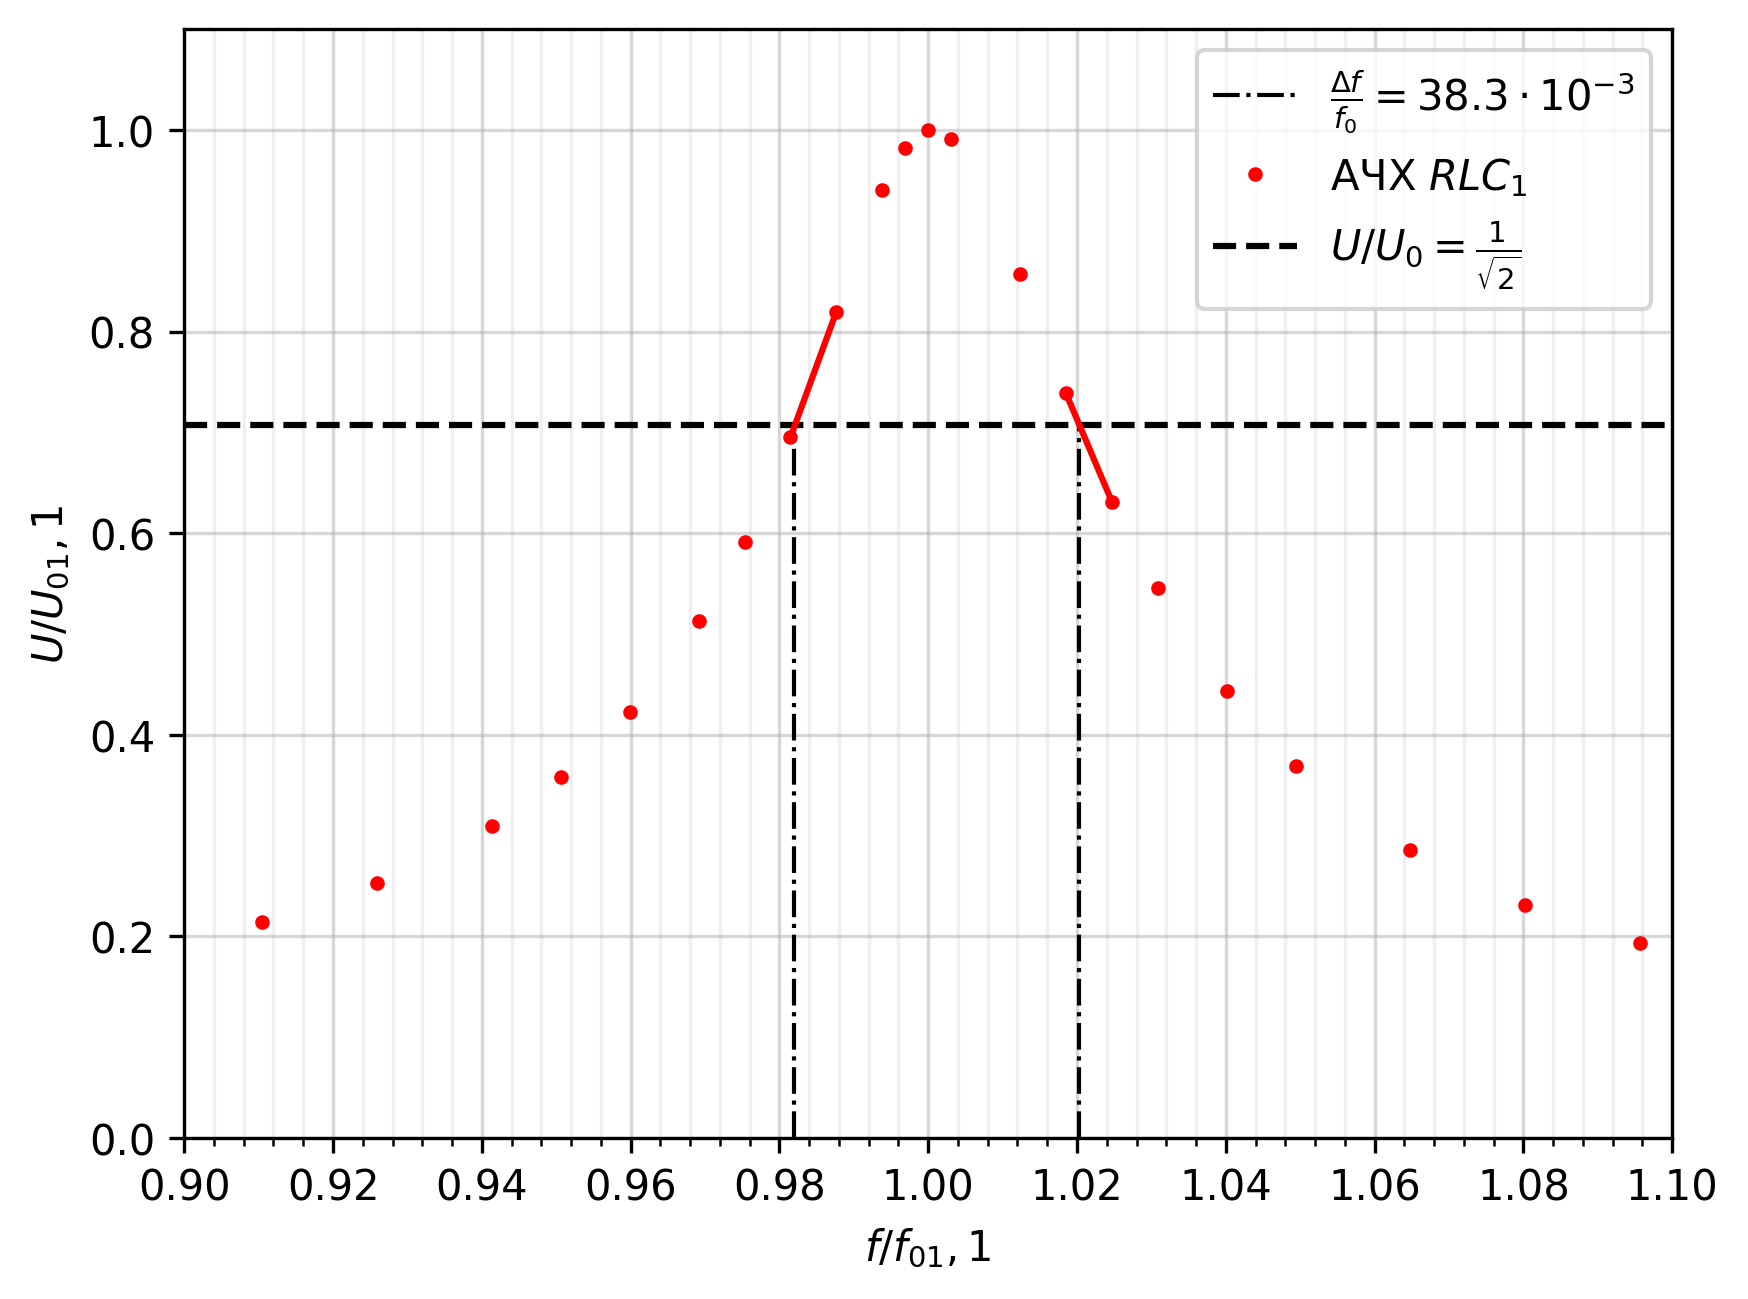
\includegraphics[width=0.8\linewidth]{afc1.png}
  \caption{АЧХ 1-го колебательного контура с уровнем $-3.5~\mathrm{dB}$}
\end{figure}

\begin{figure}[H]
  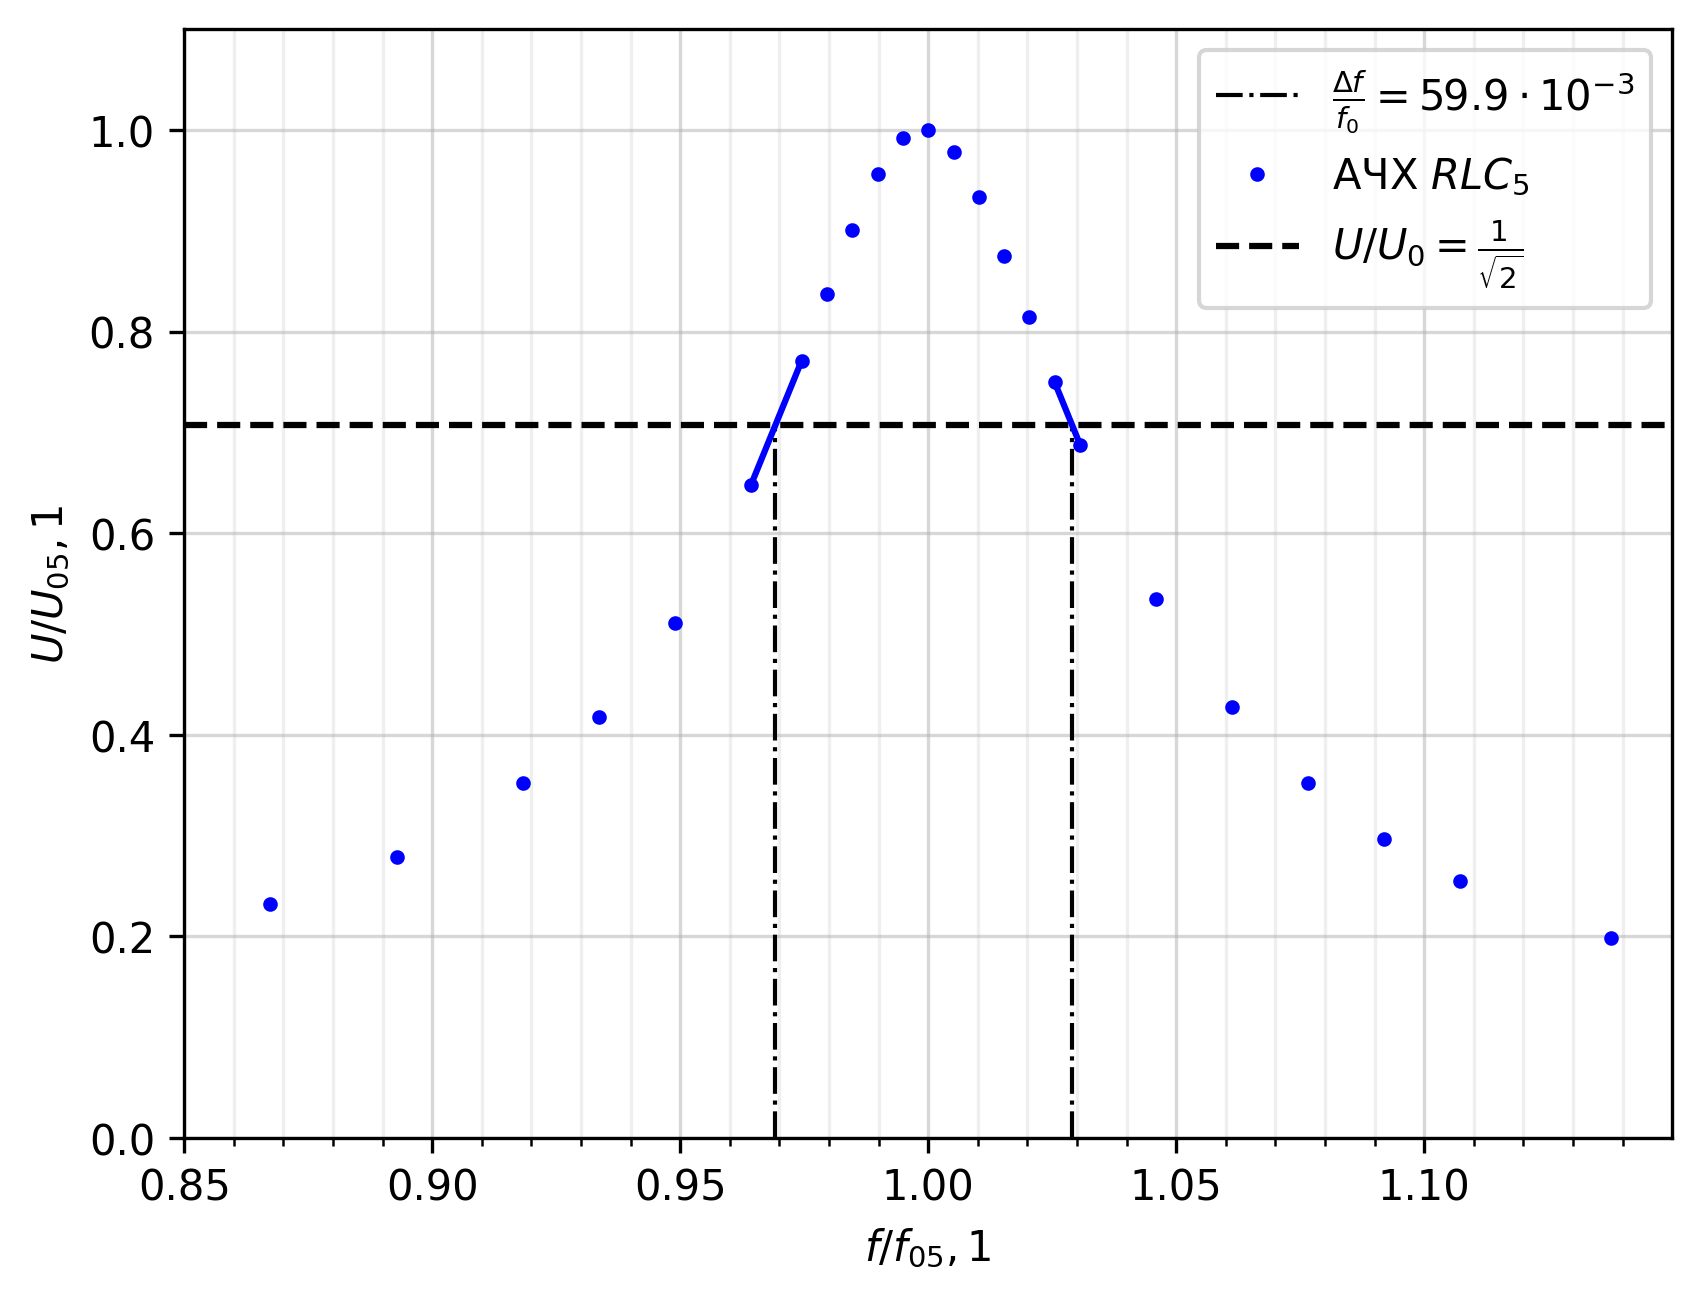
\includegraphics[width=0.8\linewidth]{afc5.png}
  \caption{АЧХ 5-го колебательного контура с уровнем $-3.5~\mathrm{dB}$}
\end{figure}

\newpage
По ширине резонансного пика на уровне в $-3.5~\mathrm{dB}$ найдем добротности контуров.
$$Q_1 = \dfrac{1}{38.3\cdot 10^{-3}} \approx 26.1$$
$$Q_5 = \dfrac{1}{59.9\cdot 10^{-3}} \approx 16.7$$

Перейдём к АЧХ.

\begin{figure}[H]
  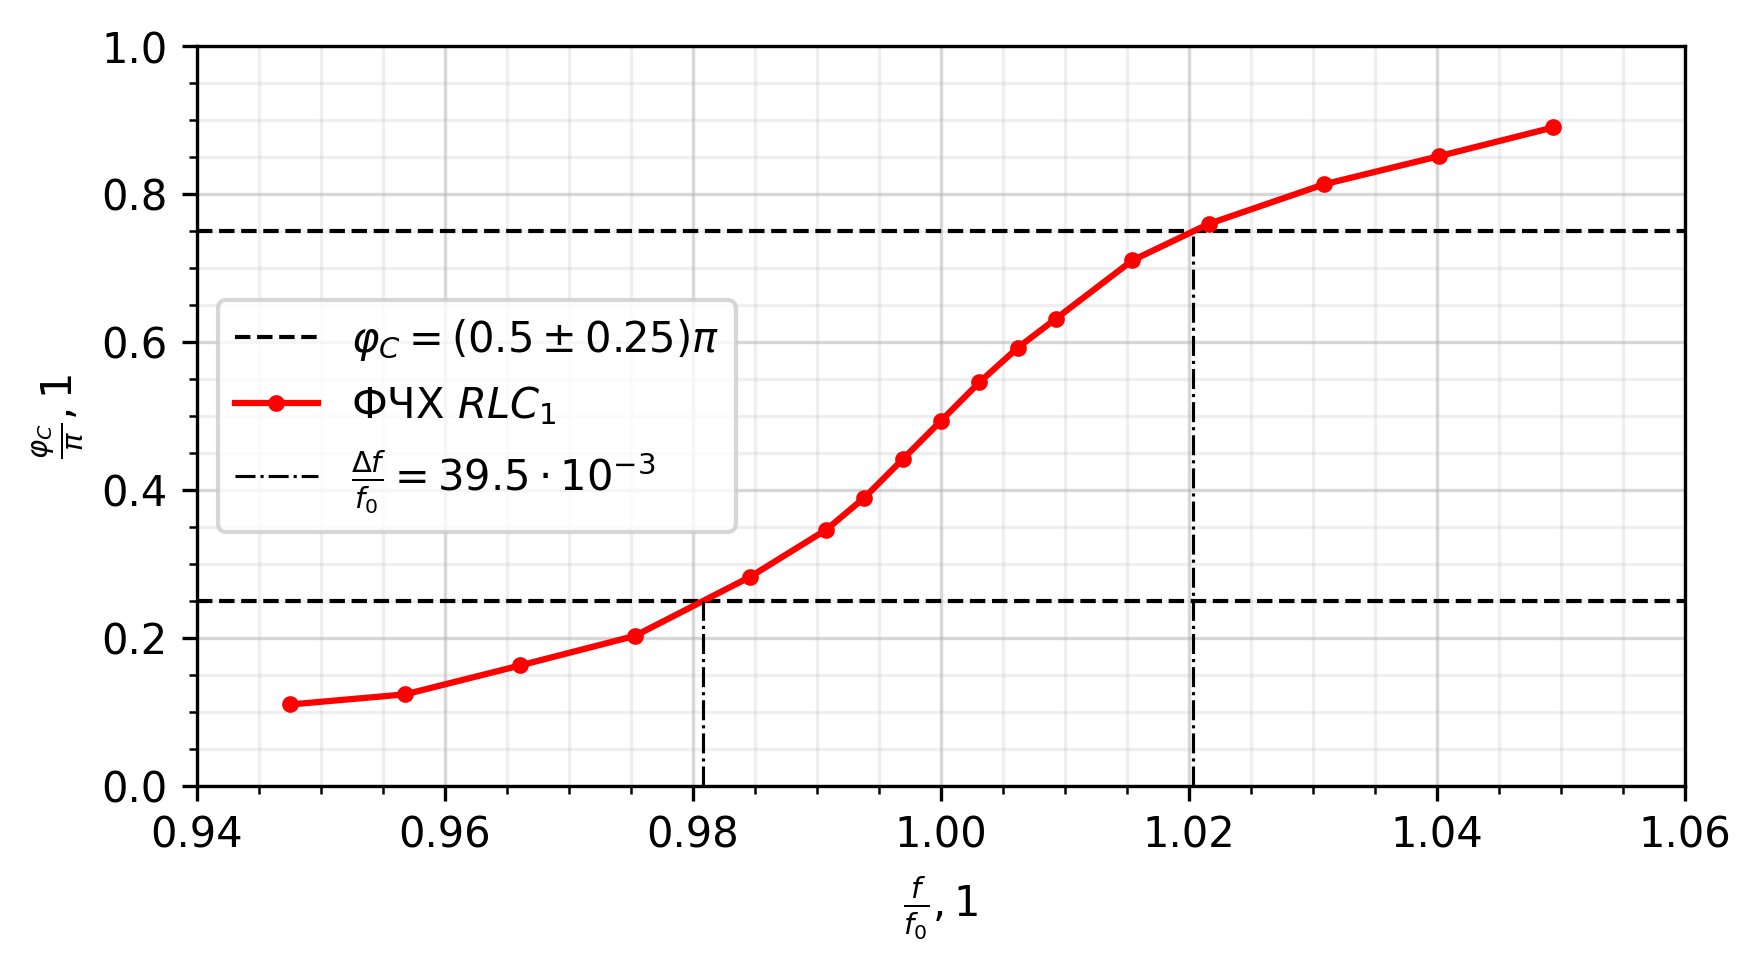
\includegraphics[width=0.8\linewidth]{pfc1.png}
  \caption{ФЧХ 1-го колебательного контура с уровнями $(0.5\pm0.25)$}
\end{figure}
\vspace{-5mm}
\begin{figure}[H]
  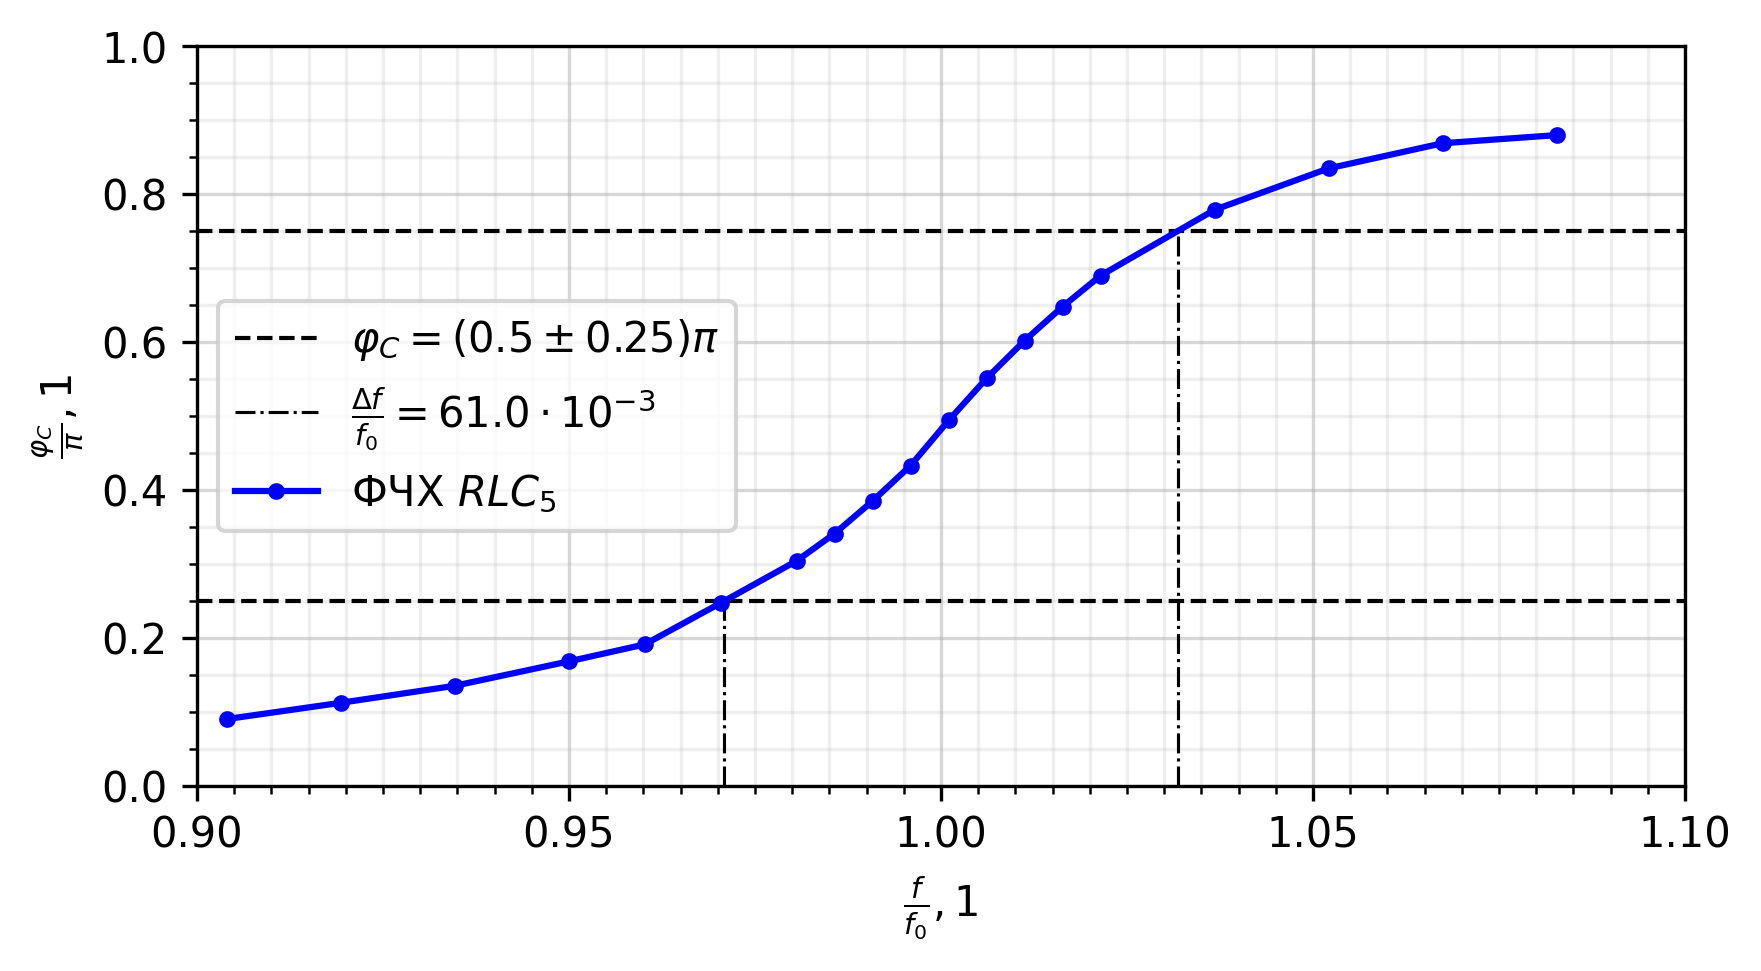
\includegraphics[width=0.8\linewidth]{pfc5.png}
  \caption{ФЧХ 5-го колебательного контура с уровнями $(0.5\pm0.25)$}
\end{figure}

Погрешность определения фазы составляет $\approx \pm 1\%$ (отношение сдвига синусоид на экране осциллографа с точностью $\pm 0.1 \text{дел.}$ к длине полуволны $\approx 10 \text{дел.}$), что примерно равно вертикальному размеру маркера на графике, поэтому кресты погрешности не наносятся.

Для этих данных получаются следующие значения добротностей:
$$Q_1 = \dfrac{1}{39.5\cdot 10^{-3}}\approx 25.3$$
$$Q_5 = \dfrac{1}{61.0\cdot 10^{-3}}\approx 16.4$$

\newpage
\begin{figure}[H]
  \centering
  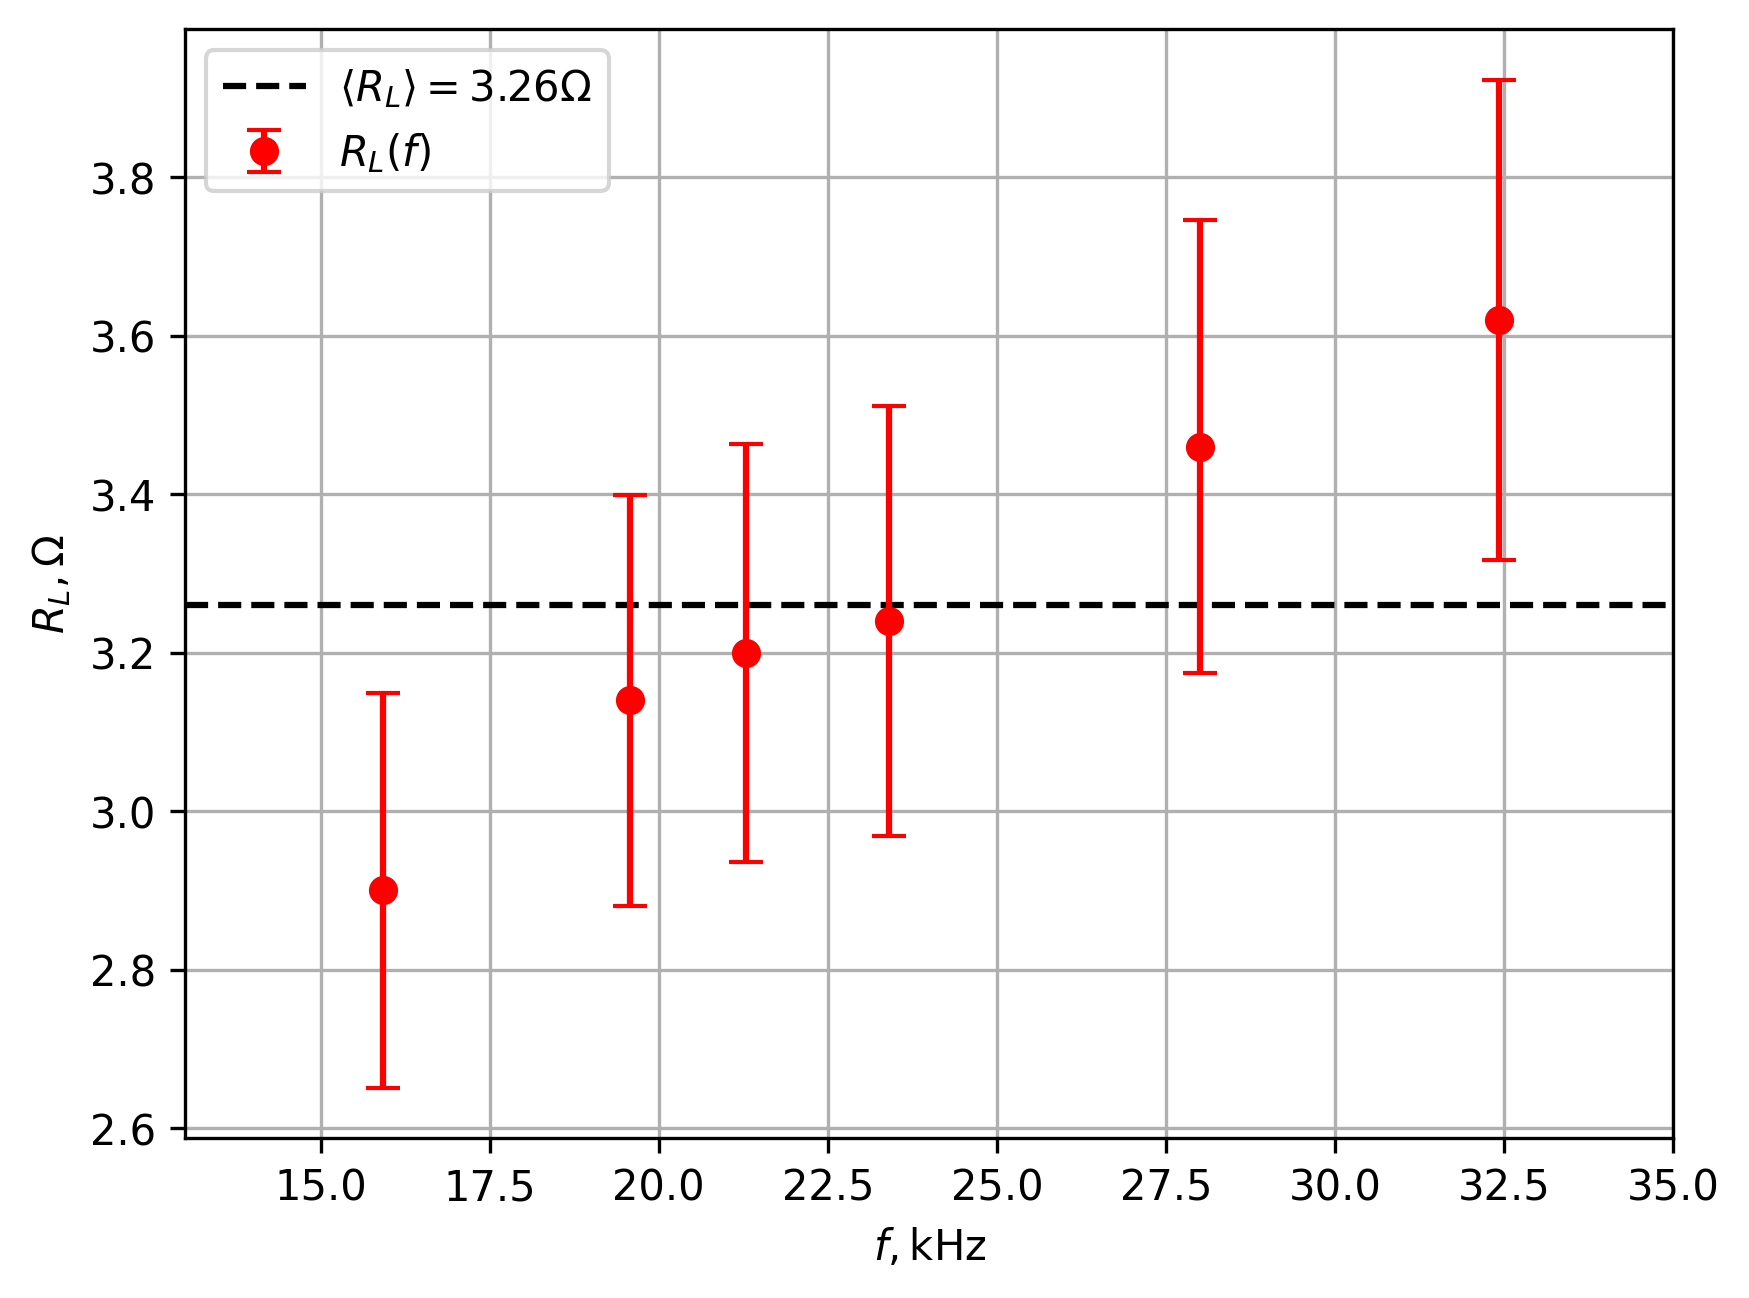
\includegraphics[width = 0.8\linewidth]{rl.png}
  \caption{Полученные результаты для зависимости $R_L$ от частоты}
  \label{rl}
\end{figure}

Здесь погрешность $R_L$ определеяется двумя наиболее важными погрешностями: случайной (посчитана в \textit{табл. \ref{dataall}}) и небольшим значением $R_S$, верхняя граница которого определялась из заводских характеристик. Таким образом, $\sigma (R_L) \approx \sqrt{\sigma(R_L)_{сл}^2 + R_{S_{max}}^2}$.


\section{Обсуждение результатов}
\begin{table}[H]
  \begin{tabular}{|l|r|r|r|r|r|}
    \hline
    & \multicolumn{1}{l|}{Высота пика} & \multicolumn{1}{l|}{АЧХ} & \multicolumn{1}{l|}{ФЧХ} & \multicolumn{1}{l|}{Среднее} & \multicolumn{1}{l|}{$\Delta(Q)_{max}$} \\ \hline
    $Q_1$ & 27.8                             & 26.1                     & 25.3                     & 26.4                         & 2.5                              \\ \hline
    $Q_5$ & 18.0                             & 16.7                     & 16.4                     & 17.0                         & 1.6                              \\ \hline
  \end{tabular}
\end{table}

Как видно из таблицы, разброс полученных значений добротности не превышает 10\%, что является хорошим результатом для величины приблизительного характера.

По графику $R_L (f)$ (\textit{рис. \ref{rl}}) видно, что крайние значения $R_L$ достоверно не совпадают со средним, при этом прослеживается линейный тренд на увеличение сопротивления с частотой. Объяснением этому явлению может служить влияние скин-эффекта, который увеличивает эффективное сопротивление единицы длины проводника из-за <<вытеснения>> плотности тока из центра провода.
\section{Выводы}
Поставленные цели работы достигнуты. С высокой точностью измерена индуктивность контура $L = (972 \pm 3)~\mathrm{\mu H}$. Сняты АЧХ и ФЧХ контуров при разных ёмкостях, разными способами с хорошей повторяемостью оценена добротность контуров. Обнаружена возрастающая зависимость активной части импеданса катушки индуктивности от частоты.

\newpage
\section{Приложение 1}

\begin{minipage}{0.45\linewidth}
  \begin{table}[H]
    \begin{tabular}{|ll|ll|}
      \hline
      \multicolumn{2}{|c|}{$RLC_1$}                                 & \multicolumn{2}{c|}{$RLC_5$}                                 \\ \hline
      \multicolumn{1}{|l|}{$f, \mathrm{kHz}$} & $U_C, \mathrm{V}$ & \multicolumn{1}{l|}{$f, \mathrm{kHz}$} & $U_C, \mathrm{V}$ \\ \hline
      \multicolumn{1}{|l|}{20.0}              & 0.0853            & \multicolumn{1}{l|}{10.0}              & 0.0715            \\ \hline
      \multicolumn{1}{|l|}{24.0}              & 0.1165            & \multicolumn{1}{l|}{13.0}              & 0.0943            \\ \hline
      \multicolumn{1}{|l|}{27.0}              & 0.1705            & \multicolumn{1}{l|}{15.0}              & 0.1268            \\ \hline
      \multicolumn{1}{|l|}{28.0}              & 0.2044            & \multicolumn{1}{l|}{16.0}              & 0.1565            \\ \hline
      \multicolumn{1}{|l|}{29.0}              & 0.2572            & \multicolumn{1}{l|}{17.0}              & 0.2081            \\ \hline
      \multicolumn{1}{|l|}{29.5}              & 0.2964            & \multicolumn{1}{l|}{17.5}              & 0.2507            \\ \hline
      \multicolumn{1}{|l|}{30.0}              & 0.3502            & \multicolumn{1}{l|}{18.0}              & 0.3163            \\ \hline
      \multicolumn{1}{|l|}{30.5}              & 0.4285            & \multicolumn{1}{l|}{18.3}              & 0.3753            \\ \hline
      \multicolumn{1}{|l|}{30.8}              & 0.4947            & \multicolumn{1}{l|}{18.6}              & 0.4590            \\ \hline
      \multicolumn{1}{|l|}{31.1}              & 0.5843            & \multicolumn{1}{l|}{18.9}              & 0.5822            \\ \hline
      \multicolumn{1}{|l|}{31.4}              & 0.7099            & \multicolumn{1}{l|}{19.1}              & 0.6928            \\ \hline
      \multicolumn{1}{|l|}{31.6}              & 0.8178            & \multicolumn{1}{l|}{19.2}              & 0.7521            \\ \hline
      \multicolumn{1}{|l|}{31.8}              & 0.9611            & \multicolumn{1}{l|}{19.3}              & 0.8089            \\ \hline
      \multicolumn{1}{|l|}{32.0}              & 1.1336            & \multicolumn{1}{l|}{19.4}              & 0.8593            \\ \hline
      \multicolumn{1}{|l|}{32.2}              & 1.3010            & \multicolumn{1}{l|}{19.5}              & 0.8915            \\ \hline
      \multicolumn{1}{|l|}{32.3}              & 1.3578            & \multicolumn{1}{l|}{19.6}              & 0.8984            \\ \hline
      \multicolumn{1}{|l|}{32.4}              & 1.3826            & \multicolumn{1}{l|}{19.7}              & 0.8791            \\ \hline
      \multicolumn{1}{|l|}{32.5}              & 1.3712            & \multicolumn{1}{l|}{19.8}              & 0.8388            \\ \hline
      \multicolumn{1}{|l|}{32.8}              & 1.1853            & \multicolumn{1}{l|}{19.9}              & 0.7862            \\ \hline
      \multicolumn{1}{|l|}{33.0}              & 1.0216            & \multicolumn{1}{l|}{20.0}              & 0.7319            \\ \hline
      \multicolumn{1}{|l|}{33.2}              & 0.8730            & \multicolumn{1}{l|}{20.1}              & 0.6734            \\ \hline
      \multicolumn{1}{|l|}{33.4}              & 0.7547            & \multicolumn{1}{l|}{20.2}              & 0.6180            \\ \hline
      \multicolumn{1}{|l|}{33.7}              & 0.6130            & \multicolumn{1}{l|}{20.5}              & 0.4808            \\ \hline
      \multicolumn{1}{|l|}{34.0}              & 0.5105            & \multicolumn{1}{l|}{20.8}              & 0.3840            \\ \hline
      \multicolumn{1}{|l|}{34.5}              & 0.3948            & \multicolumn{1}{l|}{21.1}              & 0.3160            \\ \hline
      \multicolumn{1}{|l|}{35.0}              & 0.3195            & \multicolumn{1}{l|}{21.4}              & 0.2663            \\ \hline
      \multicolumn{1}{|l|}{35.5}              & 0.2671            & \multicolumn{1}{l|}{21.7}              & 0.2294            \\ \hline
      \multicolumn{1}{|l|}{36.0}              & 0.2288            & \multicolumn{1}{l|}{22.3}              & 0.1782            \\ \hline
      \multicolumn{1}{|l|}{36.5}              & 0.1997            & \multicolumn{1}{l|}{23.0}              & 0.1402            \\ \hline
      \multicolumn{1}{|l|}{37.0}              & 0.1768            & \multicolumn{1}{l|}{24.0}              & 0.1063            \\ \hline
      \multicolumn{1}{|l|}{38.0}              & 0.1433            & \multicolumn{1}{l|}{26.0}              & 0.0705            \\ \hline
      \multicolumn{1}{|l|}{39.0}              & 0.1201            & \multicolumn{1}{l|}{28.0}              & 0.0459            \\ \hline
      \multicolumn{1}{|l|}{42.0}              & 0.0800            & \multicolumn{2}{l|}{\multirow{2}{*}{}}                     \\ \cline{1-2}
      \multicolumn{1}{|l|}{45.0}              & 0.0597            & \multicolumn{2}{l|}{}                                      \\ \hline
    \end{tabular}
    \caption{АЧХ, данные}
  \end{table}
\end{minipage}
\begin{minipage}{0.45\linewidth}
  \begin{table}[H]
    \begin{tabular}{|ll|ll|}
      \hline
      \multicolumn{2}{|c|}{$RLC_1$}                               & \multicolumn{2}{c|}{$RLC_5$}                                 \\ \hline
      \multicolumn{1}{|l|}{$f, \mathrm{kHz}$} & $\varphi_C/\pi$ & \multicolumn{1}{l|}{$f, \mathrm{kHz}$} & $U_C, \mathrm{V}$ \\ \hline
      \multicolumn{1}{|l|}{30.7}              & 0.110           & \multicolumn{1}{l|}{17.7}              & 0.090             \\ \hline
      \multicolumn{1}{|l|}{31.0}              & 0.124           & \multicolumn{1}{l|}{18.0}              & 0.112             \\ \hline
      \multicolumn{1}{|l|}{31.3}              & 0.163           & \multicolumn{1}{l|}{18.3}              & 0.135             \\ \hline
      \multicolumn{1}{|l|}{31.6}              & 0.203           & \multicolumn{1}{l|}{18.6}              & 0.168             \\ \hline
      \multicolumn{1}{|l|}{31.9}              & 0.282           & \multicolumn{1}{l|}{18.8}              & 0.191             \\ \hline
      \multicolumn{1}{|l|}{32.1}              & 0.346           & \multicolumn{1}{l|}{19.0}              & 0.247             \\ \hline
      \multicolumn{1}{|l|}{32.2}              & 0.390           & \multicolumn{1}{l|}{19.2}              & 0.304             \\ \hline
      \multicolumn{1}{|l|}{32.3}              & 0.442           & \multicolumn{1}{l|}{19.3}              & 0.341             \\ \hline
      \multicolumn{1}{|l|}{32.4}              & 0.494           & \multicolumn{1}{l|}{19.4}              & 0.385             \\ \hline
      \multicolumn{1}{|l|}{32.5}              & 0.546           & \multicolumn{1}{l|}{19.5}              & 0.433             \\ \hline
      \multicolumn{1}{|l|}{32.6}              & 0.592           & \multicolumn{1}{l|}{19.6}              & 0.494             \\ \hline
      \multicolumn{1}{|l|}{32.7}              & 0.632           & \multicolumn{1}{l|}{19.7}              & 0.551             \\ \hline
      \multicolumn{1}{|l|}{32.9}              & 0.711           & \multicolumn{1}{l|}{19.8}              & 0.602             \\ \hline
      \multicolumn{1}{|l|}{33.1}              & 0.760           & \multicolumn{1}{l|}{19.9}              & 0.648             \\ \hline
      \multicolumn{1}{|l|}{33.4}              & 0.813           & \multicolumn{1}{l|}{20.0}              & 0.690             \\ \hline
      \multicolumn{1}{|l|}{33.7}              & 0.851           & \multicolumn{1}{l|}{20.3}              & 0.779             \\ \hline
      \multicolumn{1}{|l|}{34.0}              & 0.890           & \multicolumn{1}{l|}{20.6}              & 0.835             \\ \hline
      \multicolumn{2}{|l|}{\multirow{2}{*}{}}                   & \multicolumn{1}{l|}{20.9}              & 0.869             \\ \cline{3-4}
      \multicolumn{2}{|l|}{}                                    & \multicolumn{1}{l|}{21.2}              & 0.880             \\ \hline
    \end{tabular}
    \caption{ФЧХ, данные}
  \end{table}

\end{minipage}

\newpage

\begin{figure}[H]
  \begin{tikzpicture}[scale=0.8]
    \draw [step=1, dashed, very thin] (-0.5, -16) grid (2.5, 16);
    \draw [->, thick] (0,0) -- (2,0) node [anchor=south west] {$\hat{\EDS}$};
    \draw [->, very thick] (0,0) -- (1.1,0) node [anchor=south west] {$\hat{U_R}$};
    \draw [->, very thick] (0,0) -- (0.9,15.2) node [anchor=south west] {$\hat{U_L}$};
    \draw [->, very thick] (0,0) -- (0,-15.2) node [anchor=south west] {$\hat{U_C}$};
    \draw (0.5, 0) arc (0:63.4:0.5);
    \draw (35:0.75) node {$\delta$};
    \foreach \x in {-15, -10, -5, 0, 5, 10, 15}{
      \draw (-1, \x) node {\x};
    }
  \end{tikzpicture}
\end{figure}

\end{document}
